\section{Double-counting the evidence}

\begin{enumerate}
\item Consider the two class problem where class label $y
  \in \{T, F\}$ and each training example $X$ has 2 binary attributes
  $X_1, X_2 \in \{T, F\}$. How many parameters will you \emph{need} to
  know/evaluate if you are to classify an example using the Naive
  Bayes classifier?  Keep in mind that since the probability of all
  possible events has to sum to 1, knowing the probabilities of all
  except one event implies knowledge of the final event's probability
  already.  (Don't include such final events in your count.)
  \\
  \\{\bf ANS: }
  We need four parameters to use this Naive Bayes classifier.
  \begin{align*}
  P(X_1 = T | Y = T)\\
  P(X_2 = T | Y = T)\\
  P(X_1 = T | Y = F)\\
  P(X_2 = T | Y = F)\\
  \end{align*}
  

\item Let the class prior be $\Pr(Y=T)=0.5$ and also let
  $\Pr(X_1=T \mid Y=T) = 0.8$, $\Pr(X_1=F \mid Y=F) = 0.7$, $\Pr(X_2=T
  \mid Y=T) = 0.5$, and $\Pr(X_2=F \mid Y=F) = 0.9$. (\emph{Note:} Questions 3.2 - 3.4 all use these probabilities.) So, attribute
  $X_1$ provides slightly stronger evidence about the class label than
  $X_2$.  Assume $X_1$ and $X_2$ are truly independent given
  $Y$. Write down the Naive Bayes {\bf decision rule} given $X_1=x_1$
  and $X_2=x_2$.  Write your answer as a table listing the value of
  the decision, call it $f(X_1, X_2)$, for each of the 4 settings for
  $X_1, X_2$.
\\
\\{\bf ANS:} 
Let's first write out the decision rule of Naive Bayes
\[
\frac{P(Y=T)\prod_{i=1}^n P(X_i|Y = T)}{P(Y=F)\prod_{i=1}^n P(X_i|Y=F)} \geq 1
\]
If the inequality above holds true, Naive Bayes will return Y = T\\
Following is a table of the 4 possible scenarios:\\
\\
\begin{center}
\begin{tabular}{| >{$}l<{$} | >{$}l<{$} | >{$}l<{$}|}
\hline
X_2/X_1 & X_1 = T                                             & X_1 = F\\ \hline
X_2 = T & \frac{(0.5)(0.8)(0.5)}{(0.5)(0.3)(0.1)} = 13.3 > 1  & \frac{(0.5)(0.8)(0.5)}{(0.5)(0.3)(0.9)} = 1.48 > 1\\
\hline
X_2 = F & \frac{(0.5)(0.2)(0.5)}{(0.5)(0.7)(0.1)} = 1.42 > 1  & \frac{(0.5)(0.2)(0.5)}{(0.5)(0.7)(0.9)} = 0.158 <1\\ \hline
\end{tabular}
\end{center}
such results in the following truth table:
\\
\begin{center}
\begin{tabular}{| >{$}l<{$} | >{$}l<{$} | >{$}l<{$}|}
\hline
X_2/X_1 & X_1 = T                                             & X_1 = F\\ \hline
X_2 = T & T  & T\\
\hline
X_2 = F & T  & F\\ \hline
\end{tabular}
\end{center}
  
\item For the Naive Bayes decision function $f(X_1, X_2)$,
  the error rate is:
  \begin{equation*}
    \sum_{X_1,X_2,Y} \ind{Y \ne f(X_1,X_2)}P(X_1, X_2, Y).
  \end{equation*}
  For this question, we will assume that the true data distribution is
  exactly the same as the Naive Bayes distribution, so we can write
  $P(X_1, X_2, Y)$ as $P(Y)P(X_1 \mid Y)P(X_2 \mid Y)$.

  \begin{enumerate}
    \item  Show that if Naive Bayes uses both attributes,
      $X_1$ and $X_2$, the error rate is $0.235$.
  \\{\bf ANS:}
  There are four scenarios which gives me an error:
  \begin{align*}
  P(Y = F, X_1 = T, X_2 = T) =&\; P(Y = F)P(X_1 = T \mid Y = F)P(X_2 = T \mid Y = F) = (0.3)(0.1)(0.5) = 0.015\\
  P(Y = F, X_1 = F, X_2 = T) =&\; P(Y = F)P(X_1 = F \mid Y = F)P(X_2 = T \mid Y = F) = (0.7)(0.1)(0.5) = 0.035\\
  P(Y = F, X_1 = T, X_2 = F) =&\; P(Y = F)P(X_1 = T \mid Y = F)P(X_2 = F \mid Y = F) = (0.3)(0.9)(0.5) = 0.135\\
  P(Y = T, X_1 = F, X_2 = F) =&\; P(Y = T)P(X_1 = F \mid Y = T)P(X_2 = F \mid Y = T) = (0.7)(0.5)(0.5) = 0.05
  \end{align*}
  Sum all the probability up, we obtain:
  \[
  0.015 + 0.035 + 0.135 + 0.05 = 0.235
  \]
    \item  What is the error rate using only $X_1$?
    \\
    \\{\bf ANS:}
    Since we can just read the decision rule off of one variable, I will not compute the decision rule for part b and c.\\
    There are two scenarios which gives me an error:
    \begin{align*}
    P(Y = F, X_1 = T) =&;\ (0.3)(0.5) = 0.15\\
    P(Y = T, X_1 = F) =&;\ (0.2)(0.5) = 0.1\\   
    \end{align*}
    The error rate sums up to 0.25.

    \item  What is the error rate using only $X_2$?
    \\
    \\{\bf ANS:}
    \begin{align*}
    P(Y = F, X_2 = T) =&;\ (0.1)(0.5) = 0.05\\
    P(Y = T, X_2 = F) =&;\ (0.5)(0.5) = 0.25\\   
    \end{align*}
    The error rate sums up to 0.3.

    \item  Give a conceptual explanation for why the error rate is (choose one) lower/higher using $X_1$ and $X_2$ together as opposed to using only a single attribute.
    \\
    \\{\bf ANS:}
    In this case, the error rate is lower when both $X_1$ and $X_2$ are used.  Given that my assumptions of Naive Bayes are correct, obtaining each feature gives some additional information gain to help me predict the outcome better. 
            
  \end{enumerate}

\item Now, suppose that we create a new attribute $X_3$,
  which is an exact copy of $X_2$. So, for every training example,
  attributes $X_2$ and $X_3$ have the same value, $X_2 = X_3$.

  \begin{enumerate}
  \item Are $X_2$ and $X_3$ conditionally independent given
    $Y$? 
    \\
    \\{\bf ANS:}
    They are not conditionally independent given Y because
    \[
    P(X_3 = T | Y, X_2 = T) = 1
    \]
    If they are truely conditionally independent,
    \[
    P(X_3 = T | Y, X_2 = T) = 0.3 = P(X_3 = T | Y)
    \]
    which is untrue

  \item What is the error rate of Naive Bayes now, using
    $X_1$, $X_2$, and $X_3$? The predicted $Y$ should be computed using the (possibly incorrect) assumption of conditional independence, and the error rate should be computed using the true probabilities.

Here I will save work and space by not considering $X_2 \neq X_3$ since such scenario is impossible

\begin{center}
\begin{tabular}{| >{$}l<{$} | >{$}l<{$} | >{$}l<{$}|}
\hline
X_2/X_1 & X_1 = T                                             & X_1 = F\\ \hline
X_2 = X_3 = T & \frac{(0.5)(0.8)(0.5)(0.5)}{(0.5)(0.3)(0.1)(0.1)} = 66 > 1  & \frac{(0.5)(0.8)(0.5)(0.5)}{(0.5)(0.3)(0.9)(0.9)} = 0.822 < 1\\
\hline
X_2 = X_3 = F & \frac{(0.5)(0.2)(0.5)(0.5)}{(0.5)(0.7)(0.1)(0.1)} = 7.1 > 1  & \frac{(0.5)(0.2)(0.5)(0.5)}{(0.5)(0.7)(0.9)(0.9)} = 0.087 <1\\ \hline
\end{tabular}
\end{center}
such results in the following truth table:
\\
\begin{center}
\begin{tabular}{| >{$}l<{$} | >{$}l<{$} | >{$}l<{$}|}
\hline
X_2/X_1 & X_1 = T                                             & X_1 = F\\ \hline
X_2 = X_3 = T & T  & F\\
\hline
X_2 = X_3 = F & T  & F\\ \hline
\end{tabular}
\end{center}
Now, let's calculate the error rate, note that since $X_3 = X_2$
\[
 	 P(X_3| Y, X_2) = 1
\]
\[
	P(X_3, X_2 | Y) = P(X_2 | Y)
\]

Again, four scenarios will give me error

  \begin{align*}
  P(Y = F, X_1 = T, X_2 = T, X_3 = T) =&\; P(Y = F)P(X_1 = T \mid Y = F)P(X_2 = T \mid Y = F) \\
=&\; (0.3)(0.1)(0.5)(1) = 0.015\\
  P(Y = F, X_1 = F, X_2 = T, X_3 = T) =&\; P(Y = F)P(X_1 = F \mid Y = F)P(X_2 = T \mid Y = F) \\
=&\; (0.7)(0.1)(0.5)(1) = 0.035\\
  P(Y = T, X_1 = T, X_2 = F, X_3 = F) =&\; P(Y = T)P(X_1 = T \mid Y = T)P(X_2 = F \mid Y = T) \\
=&\; (0.8)(0.5)(0.5)(1) = 0.2\\
  P(Y = T, X_1 = F, X_2 = F, X_3 = F) =&\; P(Y = T)P(X_1 = F \mid Y = T)P(X_2 = F \mid Y = T) \\
=&\; (0.7)(0.5)(0.5) = 0.05
  \end{align*}
  The error rate sums up to be 
  \[
  0.015 + 0.2 + 0.035 + 0.05 = 0.3
  \]
    
  \end{enumerate}

\item Why does Naive Bayes perform worse with the addition
  of $X_3$?  (\emph{Hint}: What assumption does Naive Bayes make about
  the inputs?)
  \\
  \\{\bf ANS:}
  When we added $X_3$, the problem does not satisfy the assumption of Naive Bayes anymore. We can see that the decision rule essentially throws out $X_1$ and becomes the same as when we only considered $X_2$. The error rate moves torwards the error rate of only $X_2$ as the result.


\item Does logistic regression suffer from the same
  problem?  Explain why or why not.
  
{\bf ANS:}
  Logistic regression does not suffer from this problem because logistic regression makes no assumption about X.

\item : In spite of the above fact we
  will see that in some examples Naive Bayes doesn't do too
  badly. Consider the above example i.e. your features are $X_1$,
  $X_2$ which are truely independent given $Y$ and a third feature
  $X_3=X_2$.  Suppose you are now given an example with $X_1 = T$ and
  $X_2 = F$.  You are also given the probabilities $\Pr(Y=T \mid
  X_1=T)=p$ and $Pr(Y=T \mid X_2=F)=q$, and $P(Y=T) = 0.5$. (\emph{Note:} You should \textbf{not} use the probabilities from 3.2-3.4 in your solutions to the following.)

  \begin{enumerate}
    \item Prove that the decision rule is $p \ge \frac{(1-q)^2}{q^2 +
      (1-q)^2}$ by applying Bayes rule again.
	\\
  	\\{\bf ANS:}
  	Let's apply Baye's rule to first
  	\begin{align*}
  	P(X_1 | Y = T) = \frac{pP(X_1)}{0.5}\\
  	P(X_1 | Y = F) = \frac{(1-p)P(X_1)}{0.5}\\
  	P(X_2 | Y = T) = \frac{qP(X_2)}{0.5}\\
  	P(X_2 | Y = f) = \frac{(1-q)P(X_2)}{0.5}
  	\end{align*}
  	
  	As we can see, when we take the fraction of one feature given $Y = T$ and $Y = F$, the $P(X)$ and $P(Y)$ cancels out. I can then write the decision rule as follows
  	\[
  	\frac{P(Y=T) \prod_i^n P(Y=T|X_i = T)}{P(Y=F) \prod_i^n P(Y=F|X_i = F)} \geq 1
  	\]
  	gives me $Y=T$//
  	So the product ends up being
  	
  	\begin{align*}
  	\frac{pq^2}{(1-p)(1-q)^2} \geq &\; 1\\
  	pq^2 \geq &\; (1-p)(1-q)^2 \\
  	pq^2 \geq &\; (1-q)^2 - p(1-q)^2 \\
  	pq^2 + p(1-q)^2 \geq &\; (1-q)^2 \\
  	p \geq &\; \frac{(1-q)^2}{q^2 + (1-q)^2}
  	\end{align*}


    \item What is the true decision rule?
\\
\\{\bf ANS:} The true decision rule can be obtained by simply taking out double counting
\[
p \geq \frac{(1-q)}{q + (1-q)} = 1-q
\]

    \item Plot the two decision boundaries (vary $q$ between $0$ and
      $1$) and highlight the region where Naive Bayes makes mistakes.
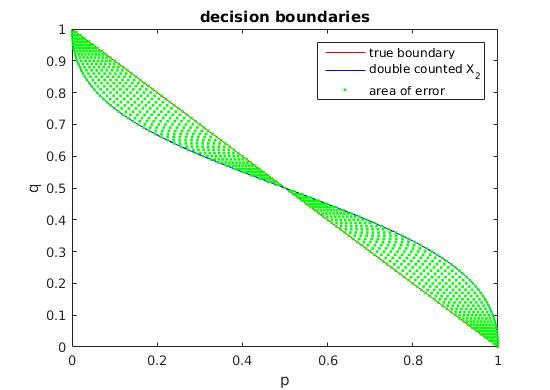
\includegraphics[scale=0.7]{decision_boundary.jpg}
      %% Don't remove the empty line below.  Compilation will fail.
      
  \end{enumerate}
\end{enumerate}
